%*****************************************
\chapter{Related Work}\label{ch:related_work}
%*****************************************
%\setcounter{figure}{10}
% \NoCaseChange{Homo Sapiens}

%BEGIN: SIMACT
\section{SIMACT: a 3D Open Source Smart Home Simulator for Activity Recognition with Open Database and Visual Editor}\label{sec:simact}

SIMACT is a flexible 3D smart home infrastructure simulator, developed in Java, specifically designed to help researchers working in the field of activity recognition \cite{bouchard2012simact}. The simulator is released as open-source \cite{bouchard:simact:Online} under GPLv3 \cite{gpl:v3}.\\

This work is specifically focused on the interaction between an agent and the surrounding environment in the smart house. It is built to reproduce everyday life scenarios, on a step-by-step basis. Entire scenarios and interactions can be designed only by writing using scripts and visual editors, without having to write one line of code.\\

The simulator is built entailer on Java based technologies. The GUI is based on the swing library, while the 3D renderer is based on the Java Monkey Engine\footnote{\url{http://jmonkeyengine.org/}}. For the 3D design, they have used a modeling tool for house design and interior accessories from Google called SketchUp \cite{sketchup:online}. This comes with a great advantage as SketchUp's community maintains a huge library of free 3D models, where one can find almost any accessory that would fit in a home.\\

To further detail, I will briefly discuss the on the system's architecture, as illustrated in Figure \ref{fig:simact_architecture}.

\begin{figure}[H]
	\centering
	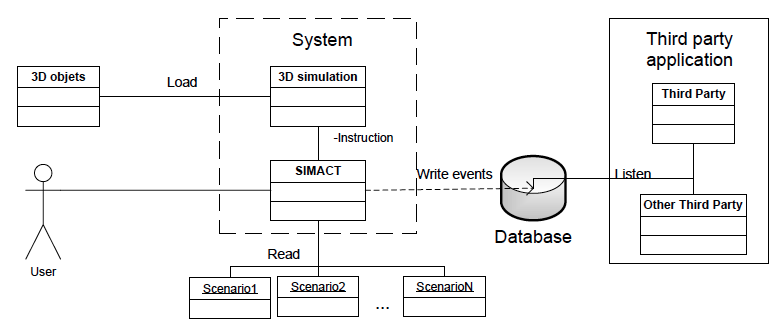
\includegraphics[width=\linewidth]{gfx/Chapter2/simact_architecture}
	\caption{SIMACT: System Architecture}
	\label{fig:simact_architecture}
\end{figure}

To create a custom simulation, a researcher starts out by defining the environment, by defining the object models contained within. The simulator loads these definitions to create the virtual model of the environment and to initialize the 3D simulator. To define the interaction with the habitat, the researcher provides the simulator with an XML file defining the interaction scenario. The scenario is defined as a sequence of steps, which is read, interpreted and execute by the simulator (it plays the role of an interpreter). As the steps are executed and the environment gets modified by these actions, the generated events are written into a database. Further, third party applications can communicate with the database to retrieve data in real-time, which can be used in the logic of the application.\\

A snapshot of the simulation tool in action is depicted in Figure \ref{fig:simact_simulation_tool}.

\begin{figure}[H]
	\centering
	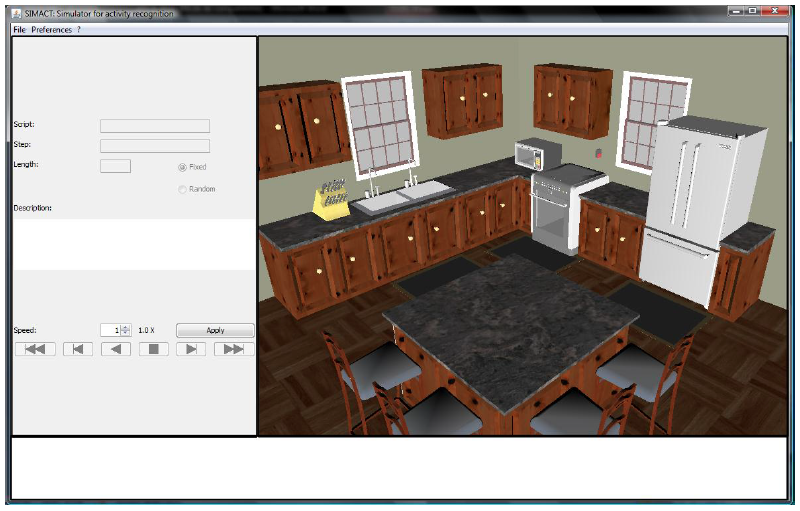
\includegraphics[width=\linewidth]{gfx/Chapter2/simact_simulation_tool}
	\caption{SIMACT: Simulation Tool in Action}
	\label{fig:simact_simulation_tool}
\end{figure}

This tool provides a powerful and reusable simulation environment, with a strong platform worth considering as basis for the simulator I am targeting to develop. My only concern is that I have not been able to determine the complexity of adding support for device simulation, as the main target of SIMACT is interaction with the physical environment.\\

In conclusion, I will allocate some time during the system design process to analyze in detail if building on top of SIMACT would be possible.

%END: SIMACT

%BEGIN: DiaSim 
\section{DiaSim: A Parameterized Simulator for Pervasive Computing Applications}\label{sec:ubiwise}

DiaSim is a Java based simulator for pervasive computing applications based on sensors and actuators \cite{bruneau2013diasim}. In this project, the simulation process starts out by defining a high-level description of the target pervasive computing environment, in a domain specific language: DiaSpec. Part of this definition are \emph{classes of entities} and \emph{data types} which can be exchanged by the entities. Based on this definition, DiaGen produces a customized \emph{programming framework} and an \emph{emulation layer}.\\

\begin{figure}[H]
	\centering
	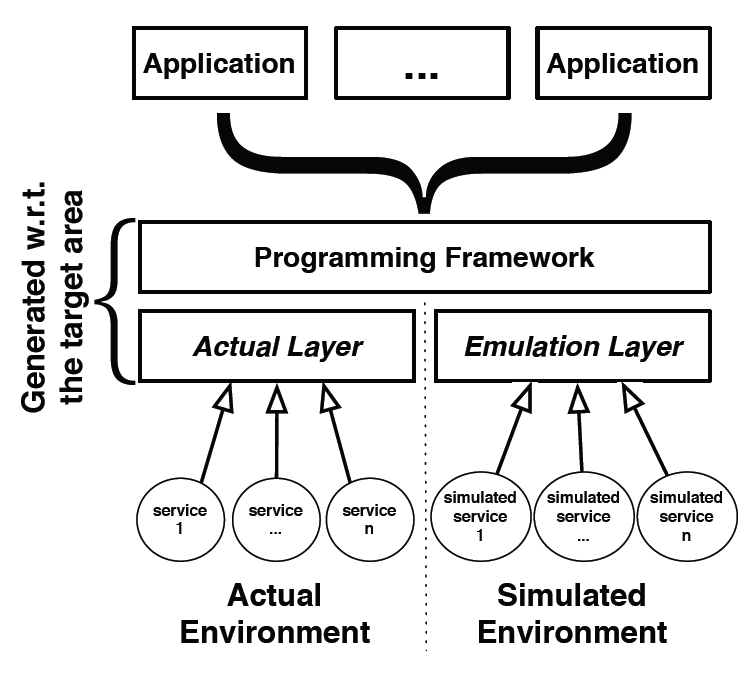
\includegraphics[width=\linewidth]{gfx/Chapter2/diasim_layered_architecture}
	\caption{DiaSim layered architecture}
	\label{fig:diasim_architecture}
\end{figure}

As depicted in Figure \ref{fig:diasim_architecture}, the simulator has a modular, layered architecture. Applications written using the generated programming framework, can be run both in a simulated and a real-world environment. In the real environment, the data comes from real sensors, while in the simulated environment the data comes from simulated sensors in the emulation environment. Besides the components mentioned so far, DiaSim also includes a simulation renderer, enabling the researcher to visually monitor and debug the pervasive computing system.\\

I found DiaSim's simulation model inspiring and relevant, hence I will further detail on a few key concepts.\\

The core entity is called a \emph{stimuli}. This represents changes of the environment observable by the sensors in the system. Entities that generate stimuli are called \emph{stimulus producers}, producing only one type of \emph{stimulus}. The generated stimuli may trigger sensors (e.g. a motion detector) which publish events, that may in turn stimulate actuators or services. Hence, we can see a stimuli as a type of stimulus; making an analogy in object-oriented programming, stimulus would be a class, stimuli would be an instance of that class and the stimulus producer would be a factory \cite{gamma1994design}, producing instances of the stimulus class based on a certain set of rules. These rules define the evolution of the stimuli in terms of space, time and intensity (e.g. an agent moving from one location to another). Each stimulus has a type associated with it, matching the type one at least one sensor in the system.\\

\begin{figure}[H]
	\centering
	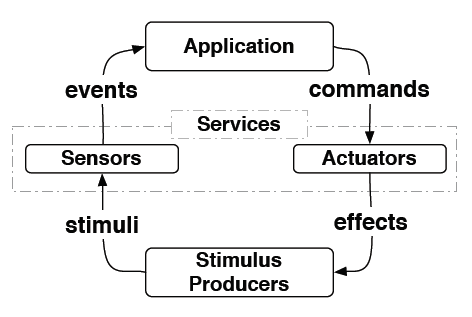
\includegraphics[width=\linewidth]{gfx/Chapter2/diasim_simulation_model}
	\caption{DiaSim simulation model}
	\label{fig:diasim_simulation_model}
\end{figure}

As illustrated in Figure \ref{fig:diasim_simulation_model}, besides stimulus producers, the simulated environment also contains simulated services; they process stimuli, perform actions and interact with other services. The two key services in this simulator are \emph{sensors} and \emph{actuators}. The interaction between services and the environment are based on one of the existing three interaction modes:
\begin{itemize}
	\item Command (one-to-one, synchronous interaction). Usually received by actuators to modify their state (e.g. on/off command for a light)
	\item Event (one-to-many, asynchronous interaction). Usually generated by sensors when they receive stimuli (e.g. a motion detector when receiving location stimuli matching its room, would generate an event containing the room's number)
	\item Session (one-to-one with information exchange over a period of time). For example, when motion from an unknown source is detected in a restricted area, an audio notification service could stream a warning audio notification to a nearby speaker service.
\end{itemize}

After thorough analysis, I found DiaSim as being a good starting point for my work. The simulation model is generic enough to host our needs and open for further modifications. Also the rendering module allows to easily visualize the simulated system and control an agent in a 2D environment. But, the system is not open source and the research team is not yet open for external collaboration.

\subsection{Siafu}
To render the simulation, DiaSim was coupled with Siafu \cite{siafu:online}, a highly customizable, open-source Java based simulator for mobile context-aware applications and services \cite{martin2006generic}. Although Siafu enables the definition of any context type, does not provide any support to simulate entities and applications.\\

Siafu was meant to be a flexible simulator. Hence, they have separated the main information sources from each other:
\begin{itemize}
	\item Agent Model. Takes decision on what a certain agent should do given it's current context and the status of surrounding entires. As a result, the model will change the properties of an agent (e.g. standing, sitting, walking etc.). A special property is the destination. This will make the agent move in the surrounding environment; movement and path finding routines are handled automatically by the simulator.
	\item World Model. Consists of an environment model, places of interest (e.g. office, rooms etc.) and global events model (e.g. holidays, happy hour at a restaurant etc.)
	\item Context Model. Manages context variables used in the simulation.
\end{itemize}

The simulated data is available in 2D graphical representation and through a web service interface.\\

I have briefly discussed about Siafu as I found relevant the way it was integrated with DiaSim. As illustrated in Figure \ref{fig:diasim_and_siafu}, the main models in DiaSim are extended from the three abstract information sources in Siafu: AgentModel, ContextModel and WorldModel. Further, the DiaSim aggregates the simulated entities and stimuli producers.

\begin{figure}[H]
	\centering
	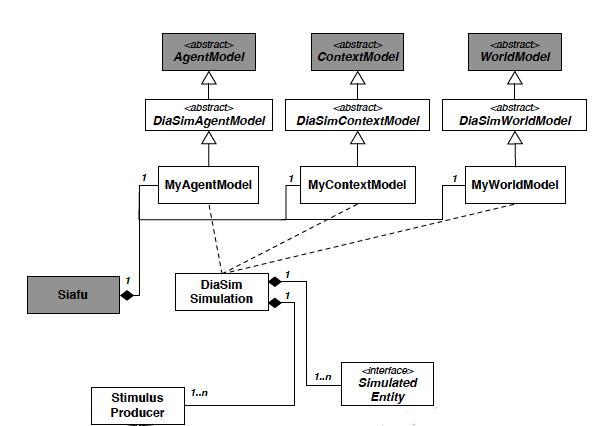
\includegraphics[width=\linewidth]{gfx/Chapter2/diasim_and_siafu}
	\caption{DiaSim and Siafu}
	\label{fig:diasim_and_siafu}
\end{figure}

Based on this approach, DiaSim managed to easily integrate a 2D simulation renderer in their work. I am considering to further analyze Siafu as a possible corner stone for our approach.
%END: DiaSim 

%BEGIN: UbiWise 
\section{UbiWise, A Simulator for Ubiquitous Computing Systems Design}\label{sec:ubiwise}

UbiWise \cite{barton2003ubiwise} is a device-centric simulator. The target of this work was to allow researchers to simulate ubiquitous computing devices\footnote{networked, context-aware devices} before physical prototypes are available. The purpose of this is to empower the researcher to write software for the device and test it from a user interaction's point of view, in the actual physical environment the device was envisioned to be used in. This project emerged from two independent simulators: UbiSim and WISE.\\

UbiSim is a 3D environment simulator, aimed at producing context information in real-time, in a close to realistic environment. To simulate the environment, they have use the Quake III Arena (Q3A)\footnote{http://www.idsoftware.com/gate.php} first person shooter gaming engine, written in the C programming language. On top of the raw simulated data outputted by Q3A, they have built a \emph{context server} which processes the simulated data and delivers meaningful context data to external applications and services. The simulator is also able to process data from sensors in the real-world, generating mixed reality together with the simulated data.\\

WISE is a 2D device interaction simulator written in Java. This allows the user to interact with the software running on the device, interacting with real-world web services and other simulated devices.\\

In the 3D physical environment, the set of simulated devices are used in a context-aware manner, reacting to physical events and contextual changes. The devices might be portable, hand-held by a virtual agent the user controls (e.g. a digital camera enhanced with Internet connectivity) or they might be static device, attached to a physical entity (e.g. a wireless enhanced picture frame). In simulated environment might detect the proximity between the devices, triggering events and allowing the software running on the device to take specific actions.\\

In the 2D environment, the set of devices are presented in desktop-alike windows and they react to mouse clicks and network events. This allows to user to directly interact with the device as he would in the real-world.\\

UbiWise was released under LGPL\cite{lgpl} offering the software to the open-source community.\\
%END: UbiWise

%BEGIN: Tatus
\section{A Testbed for Evaluating Human Interaction with Ubiquitous Computing Environments}\label{sec:tatus}

TATUS \cite{o2005testbed} is as a ubiquitous computing simulator aimed at overcoming the challenges of effectively evaluating human interaction with adaptive ubiquitous technologies. These challenges are mainly imposed by the cost and logistics of building and controlling the context in such real-life environments. In other words, TATUS is a simulator supporting research and development of adaptive software controlling ubiquitous computing environments.\\

Figure \ref{fig:tatus_overview} depicts the high-level overview of the simulator. We can identify two main components: the 3D Simulated Ubiquitous Computing Environment and the System Under Test (SUT).\\

\begin{figure}[H]
	\centering
	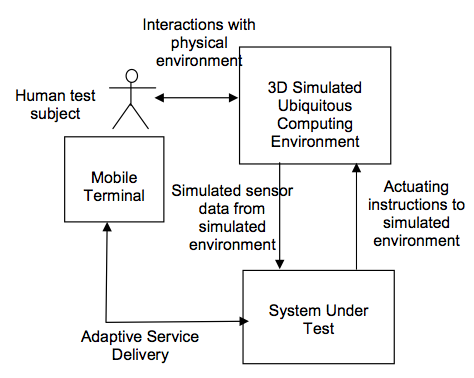
\includegraphics[width=\linewidth]{gfx/Chapter2/tatus_system_overview}
	\caption{High-level simulator overview}
	\label{fig:tatus_overview}
\end{figure}

The 3D simulator was implemented on top of the Half-Life\footnote{\url{http://www.valvesoftware.com}} Game Engine's software development kit (SDK), written in C/C++. Half-Life is a 3D first-person-shooter network game. It is implemented based on client-server architecture with multi-player capabilities (up to 32 players simultaneously). The reason for choosing this game engine was to exploit the 3D graphics engine in order to provide a realistic user experience.\\

The actual simulated environment is created using a map editor from Valve called Hammer (a drawing tool for building maps). This can be used to generate complex and realistic environments as the tool offers a wide range of graphical editing possibilities, as exemplified in Figure \ref{fig:tatus_simulated_meeting_room}. The SDK is then able to load a simulated environment's physical settings from the files generated by the map editor.\\

\begin{figure}[H]
	\centering
	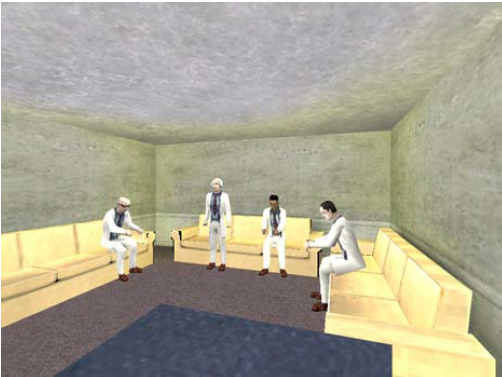
\includegraphics[width=\linewidth]{gfx/Chapter2/tatus_simulated_meeting_room}
	\caption{Simulated meeting room with multiple characters}
	\label{fig:tatus_simulated_meeting_room}
\end{figure}

To simulated sensors and actuators they have exploited a concept called \emph{Triggers} from the SDK. They are used to generate associated events based on a player's movements and location. The state of these triggers together with the agents location at a certain point in time represent the state of the simulated environment. To allow easy access to the data, the simulator exposes an API which offers both querying and modifying capabilities. Queries allow to select certain aspects of the current state based on various parameters, whereas through modifications the SUT can impose changes on the simulated environment.\\

A SUT is written as independent pieces of software. It can even run on a separate machines, while multiple SUTs can connect simultaneously to the same simulator. To allow SUTs to run on separate machines the simulator has embedded networking capabilities and communicates through messages. Outgoing messages carry state information, while incoming messages care instructions to modify the simulated environment. Moreover, to abstract out the network interaction from the SUTs, the simulator provides a Proxy making the communication from the test software's side really easy.\\

\subsection{Conclusions}

One of the main challenges in developing the simulator was that the learning curve of the SDK, in order to extend it, was difficult and time-consuming. But, as a result, they have tried to provide a flexible simulation environment where researchers can easily simulate other environments without the need to modify any SDK level code.\\

The context-awareness is limited to sensors and actuators reacting to the user's position. This is actually not that bad because in the game engine SDK the developer can extract the position of entities, determine proximity of other entities within a given radius and determine the presence of other entities within a field of view. All these data helps to implement simulations for a wide range of sensors.\\

The user control provided by the game engine is pretty advanced allowing the agent to move in any direction, crouch, jump, sit etc. This is a big plus as it adds a good sense of reality to the game.\\

Multiple users can join and experience the same simulated environment at the same time. Not all player have to be human, not-player-characters (controlled by the AI of the engine) can be present as well.\\

Unfortunately the simulator is not open-source so making it unusable for research outside the institution it was developed in.
%END: Tatus

%BEGIN: Service in Smart Homes
\section{Services inside the Smart Home: A Simulation and Visualization tool}\label{sec:services_in_smart_homes}

In this work \cite{lazovik2009services} the aim is to reduce the testing costs of smart homes. The goal was achieved by implementing a simulation and visualization tool which replaces services in a smart home with virtual stubs behaving just like the real hardware installed in a house.\\

For the implementation of virtual stubs they have employed the service-oriented computing paradigm, which is widely used to implement systems requiring high interoperability, scalability, security and reliability. One of the main advantages is that such software can seamlessly integrate other systems written in other programming languages and even deployed under different operating systems.\\

The simulation scenarios are built using Google SketchUp \cite{sketchup:online}. This was extended with a set of tools extending its visual representation of a house with virtual home interactive web services supporting SOAP messages. Further, the visualization component is written as a set of plug-ins for Google SketchUp.\\

The simulation and visualization tool allows to simulate any possible home automation scenario, with the possibility of modeling the user and its interactions with the home.
%END: Service in Smart Homes

%BEGIN: Simulation of Smart Environments
\section{Simulation of Smart Environments}\label{sec:sim_of_smart_envs}

Armac and Retkowitz developed a tool called \emph{eHomeSimulator}, which was build in order to support the simulation of smart environments, or as the authors refer to them in the present work \emph{eHomes} \cite{armac2007simulation}. The motivation behind the work is that smart environments constitute already an important research area, but building a real eHome is associated with high effort and financial costs. Therefore, the eHomeSimulator helps in abstracting out from creating buildings (the actual physical environment) and purchasing devices, allowing us to focus only on software engineering aspects and challenges involved in eHome development (e.g. developing services, deployment etc.).\\

Describing in details the eHome is out of scope, but for clarity, I will a offer a short description. Therefore, eHome is basically a framework consisting of a hardware platform (the residential gateway) and a software platform (service gateway, runs on top of the hardware platform). The devices and appliances, which make up the eHome, are connected to the hardware platform. They are of two basic types: sensors and actuators. Sensors offer contextual information like temperature, humidity etc. while actuators can change the environment's state (e.g. a speaker, a heater etc.). The hardware platform is governed by the software platform which acts as a runtime environment for eHome services. These services can be of two types: basic and integrating. Basic service are meant to control devices (e.g. a lamp driver) while the integrating services are composed of various basic service. These services are developed based on the OSGi component model \cite{allianceosgi}, imposing a highly decoupled architecture to the service model and offering high reusability of the developed services. One novelty introduced by the architecture of the framework is that service can work both with real device and simulate device.\\

The eHomeSimulator is built on top of eHome framework to allow intuitive interaction and to visually represent the state of the simulated environment. In the evaluation process of the simulator, eHome environments consist of three main elements: rooms devices and persons (agents interacting with the environment). The graphical representation is a 2D view with a view point from top, which is built up from three layers:
\begin{itemize}
	\item The bottom layer contains the graphics to represent the background (floor, walls and furniture) build up from tiles placed one next to each other.
	\item On top of the background, there is the middle layer representing the graphics of the devices. These are only static devices and they can have different colors based on their state.
	\item The top layer represents the agents interacting with the environment. They can move freely in all accessible areas, interacting with the devices.
\end{itemize}

There is a environment editor which assists in setting up a simulated environment. The process starts by designing the room, walls and furniture using Google Sketchup \cite{sketchup:online} which then is uploaded into the editor. On top of this base we can further place the devices and appliances.\\

The eHomeSimulator's architecture is based on the Model View Controller design pattern \cite{erich1995design}. The model of the system holds the data structures representing the current state of the system, the view implements the graphical representation based on the current model and the controller process the user interaction with the simulator, updating the view according to changes in the model.\\

The image depicted in Figure \ref{fig:simulated_env} displays a simulation in progress. On the right side, we can observe the agent interacting with the environment while on the left side there is a control panel displaying various context data of the current status of the system and allows to interact with nearby devices (e.g. turn on/off a lamp).

\begin{figure}[H]
	\centering
	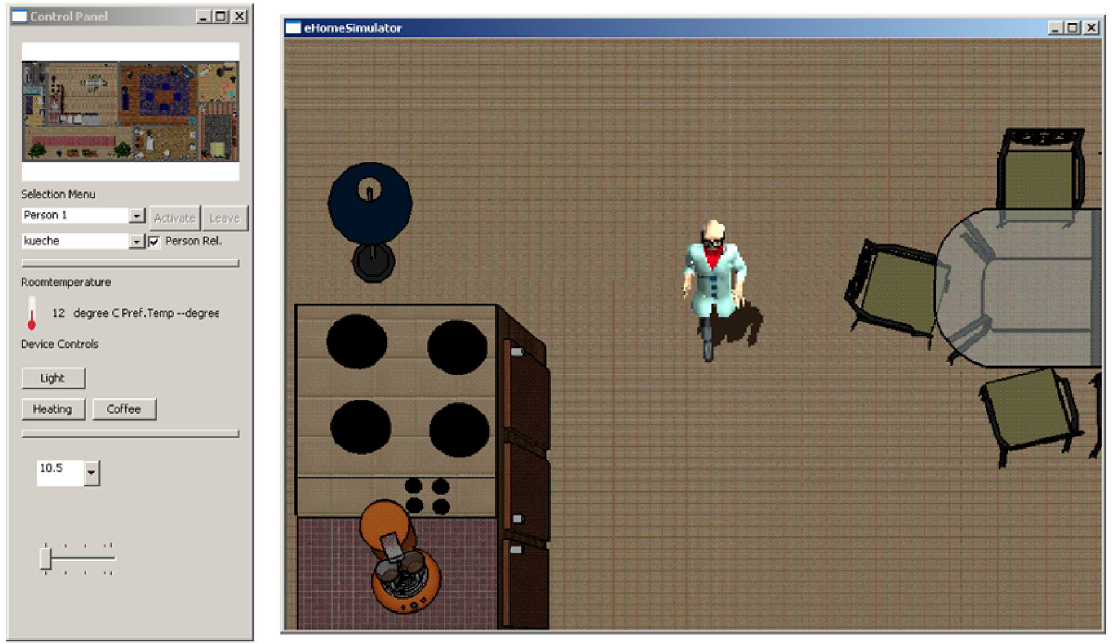
\includegraphics[width=\linewidth]{gfx/Chapter2/simulated_env}
	\caption{The GUI of the simulator}
	\label{fig:simulated_env}
\end{figure}

The eHomeSimulator has an architecture providing loose coupling between components. Also, the underlying framework's architecture offers great support for reusability of services and integration with real-life devices. The devices are trivial, offering basic interactions (e.g. on/off) and they are static (the agent can't move them). Actually, all the agent can do is move around between some given bounds and interact with some of the device. There is no support for mobility of devices and wearable device, nor is it in plan for future work. Moreover, the representation of the agent is in 2D where he can be facing 4 directions, offering no support for various states like sitting, standing etc.\\

The project is close sourced, making it impossible to extend, to reuse or to contribute to it. In conclusion, there are a few lessons to be learnt from the architectural choices made within this project.
%END: Simulation of Smart Environments